\documentclass[a4paper, 12pt]{ctexart}
% generated by Madoko, version 1.1.3
%mdk-data-line={1}


\usepackage[heading-base={2},section-num={False},bib-label={hide},fontspec={True}]{madoko2}


\begin{document}



%mdk-data-line={6}
\mdxtitleblockstart{}
%mdk-data-line={6}
\mdxtitle{\mdline{6}数字媒体技术}%mdk
\mdtitleauthorrunning{}{}\mdxtitleblockend%mdk

%mdk-data-line={7}
\section{\mdline{7}1.\hspace*{0.5em}\mdline{7}PCA}\label{sec-pca}%mdk%mdk

%mdk-data-line={8}
\subsection{\mdline{8}1.1.\hspace*{0.5em}\mdline{8}背景:}\label{section}%mdk%mdk

%mdk-data-line={9}
\noindent\mdline{9}在多元统计分析中,主成分分析(英语:Principal components analysis,PCA)是一种分析、简化数据集的技术。主成分分析经常用于减少数据集的维数,同时保持数据集中的对方差贡献最大的特征。这是通过保留低阶主成分,忽略高阶主成分做到的。这样低阶成分往往能够保留住数据的最重要方面。但是,这也不是一定的,要视具体应用而定。由于主成分分析依赖所给数据,所以数据的准确性对分析结果影响很大。%mdk

%mdk-data-line={11}
\subsection{\mdline{11}1.2.\hspace*{0.5em}\mdline{11}数学定义:}\label{section}%mdk%mdk

%mdk-data-line={12}
\noindent\mdline{12}PCA的数学定义是:一个正交化线性变换,把数据变换到一个新的坐标系统中,使得这一数据的任何投影的第一大方差在第一个坐标(称为第一主成分)上,第二大方差在第二个坐标(第二主成分)上,依次类推\mdline{12}[4]\mdline{12}。
定义一个n × m的矩阵, XT为去平均值(以平均值为中心移动至原点)的数据,其行为数据样本,列为数据类别(注意,这里定义的是XT 而不是X)。则X的奇异值分解为X = WΣVT,其中m × m矩阵W是XXT的本征矢量矩阵, Σ是m × n的非负矩形对角矩阵,V是n × n的XTX的本征矢量矩阵。据此,%mdk

%mdk-data-line={16}
\mdline{16}\mdline{22}
\mdline{23}\mdline{23}
当 m \mdline{24}\textless{}\mdline{24} n − 1时,V 在通常情况下不是唯一定义的,而Y 则是唯一定义的。W 是一个正交矩阵,YT是XT的转置,且YT的第一列由第一主成分组成,第二列由第二主成分组成,依此类推。
为了得到一种降低数据维度的有效办法,我们可以利用WL把 X 映射到一个只应用前面L个向量的低维空间中去:%mdk


%mdk-data-line={86}
\noindent\mdline{86}X 的单向量矩阵W相当于协方差矩阵的本征矢量 C = X XT,\mdline{86}\mdline{86}
\mdline{87}\mdline{87}%mdk








%mdk-data-line={365}
\subsection{\mdline{365}1.3.\hspace*{0.5em}\mdline{365}算法实现一般过程:}\label{section}%mdk%mdk

%mdk-data-line={366}
\begin{enumerate}[noitemsep,topsep=\mdcompacttopsep]%mdk

%mdk-data-line={366}
\item\mdline{366}求平均值以及做normalization%mdk

%mdk-data-line={367}
\item\mdline{367}求协方差矩阵(Covariance Matrix)%mdk

%mdk-data-line={368}
\item\mdline{368}求协方差矩阵的特征根和特征向量%mdk

%mdk-data-line={369}
\item\mdline{369}选择主要成分(信息量)%mdk

%mdk-data-line={370}
\item\mdline{370}转化得到降维的数据%mdk
%mdk
\end{enumerate}%mdk

%mdk-data-line={372}
\subsection{\mdline{372}1.4.\hspace*{0.5em}\mdline{372}实验结果}\label{section}%mdk%mdk

%mdk-data-line={373}
\noindent\mdline{373}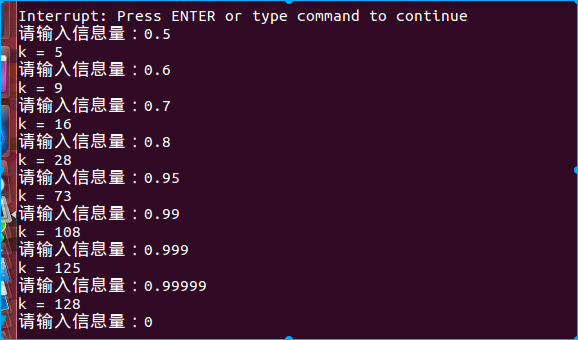
\includegraphics[keepaspectratio=true,width=\dimmin{}{\dimwidth{0.90}}]{images/PCA}{}\mdline{373}%mdk

%mdk-data-line={377}
\section{\mdline{377}2.\hspace*{0.5em}\mdline{377}JPEG压缩原理与DCT离散余弦变换}\label{sec-jpegdct}%mdk%mdk

%mdk-data-line={378}
\subsection{\mdline{378}2.1.\hspace*{0.5em}\mdline{378}背景:}\label{section}%mdk%mdk

%mdk-data-line={379}
\noindent\mdline{379}DCT变换的全称是离散余弦变换(Discrete Cosine Transform),主要用于将数据或图像的压缩,能够将空域的信号转换到频域上,具有良好的去相关性的性能。DCT变换本身是无损的,但是在图像编码等领域给接下来的量化、哈弗曼编码等创造了很好的条件,同时,由于DCT变换时对称的,所以,我们可以在量化编码后利用DCT反变换,在接收端恢复原始的图像信息。DCT变换在当前的图像分析已经压缩领域有着极为广大的用途,我们常见的JPEG静态图像编码以及MJPEG、MPEG动态编码等标准中都使用了DCT变换。%mdk

%mdk-data-line={381}
\mdline{381}\mdline{381}
\mdline{382} \mdline{382}%mdk

%mdk-data-line={384}
\subsection{\mdline{384}2.2.\hspace*{0.5em}\mdline{384}数学定义:}\label{section}%mdk%mdk

%mdk-data-line={386}
\subsubsection{\mdline{386}2.2.1.\hspace*{0.5em}\mdline{386}一维DCT变换}\label{sec-dct}%mdk%mdk

%mdk-data-line={387}
\noindent\mdline{387}一维DCT变换时二维DCT变换的基础,所以我们先来讨论下一维DCT变换。一维DCT变换共有8种形式,其中最常用的是第二种形式,
由于其运算简单、适用范围广。我们在这里只讨论这种形式,其表达式如下:%mdk

%mdk-data-line={391}
\mdline{391}\mdline{391}%mdk

%mdk-data-line={394}
\mdline{394}其中,f(i)为原始的信号,F(u)是DCT变换后的系数,N为原始信号的点可以认为是一个补偿系数,可以使DCT变换矩阵为正交矩阵。%mdk

%mdk-data-line={396}
\subsubsection{\mdline{396}2.2.2.\hspace*{0.5em}\mdline{396}二维DCT变换}\label{sec-dct}%mdk%mdk

%mdk-data-line={397}
\noindent\mdline{397}二维DCT变换其实是在一维DCT变换的基础上在做了一次DCT变换,其公式如下:%mdk

%mdk-data-line={399}
\mdline{399}\mdline{399}
\mdline{400}\mdline{400}
       由公式我们可以看出,上面只讨论了二维图像数据为方阵的情况,在实际应用中,如果不是方阵的数据一般都是补齐之后再做变换的,重构之后可以去掉补齐的部分,得到原始的图像信息,这个尝试一下,应该比较容易理解。%mdk

%mdk-data-line={403}
\mdline{403}另外,由于DCT变换高度的对称性,在使用Matlab进行相关的运算时,我们可以使用更简单的矩阵处理方式:%mdk

%mdk-data-line={405}
\mdline{405}\mdline{405}%mdk

%mdk-data-line={408}
\subsection{\mdline{408}2.3.\hspace*{0.5em}\mdline{408}JPEG压缩流程:}\label{sec-jpeg}%mdk%mdk

%mdk-data-line={409}
\begin{enumerate}[noitemsep,topsep=\mdcompacttopsep]%mdk

%mdk-data-line={409}
\item\mdline{409}以8x8的图象块为基本单位进行编码%mdk

%mdk-data-line={410}
\item\mdline{410}将RGB转换为亮度-色调-饱和度系统(YUV),并重新采样%mdk

%mdk-data-line={411}
\item\mdline{411}FDCT%mdk

%mdk-data-line={412}
\item\mdline{412}量化%mdk

%mdk-data-line={413}
\item\mdline{413}编码%mdk

%mdk-data-line={414}
\item\mdline{414}解码%mdk

%mdk-data-line={415}
\item\mdline{415}反量化%mdk

%mdk-data-line={416}
\item\mdline{416}IDCT%mdk

%mdk-data-line={417}
\item\mdline{417}图像拼接%mdk
%mdk
\end{enumerate}%mdk

%mdk-data-line={419}
\subsection{\mdline{419}2.4.\hspace*{0.5em}\mdline{419}实验结果:}\label{section}%mdk%mdk

%mdk-data-line={420}
\noindent\mdline{420}压缩率:10\mdline{420}\mdline{420}
\mdline{421}\mdline{421}%mdk

%mdk-data-line={423}
\mdline{423}\mdline{423}
压缩率:50\mdline{424}\mdline{424}
\mdline{425}\mdline{425}
\mdline{426}\mdline{426}
JPEG压缩比例,就是通过控制量化的多少来控制。比如,上面的量化矩阵Q,如果我把矩阵的每个数都double一下,那是不是会出现更多的0?!说不定都只有G(0, 0)非0,其他都是0,如果这样,那编码时就可以更省空间啦,N个0只要一个游程编码搞定,数据量超小。但也意味着,恢复时,会带来更多的误差,图像质量也会变差了。%mdk

%mdk-data-line={432}
\section{\mdline{432}3.\hspace*{0.5em}\mdline{432}Madoko}\label{sec-madoko}%mdk%mdk

%mdk-data-line={434}
\noindent\mdline{434}Madoko is a fast markdown processor for writing professional articles
with a focus on simplicity and plain text readability.%mdk

%mdk-data-line={437}
\begin{itemize}[noitemsep,topsep=\mdcompacttopsep]%mdk

%mdk-data-line={437}
\item\mdline{437}Read the\mdline{437}~\href{http://research.microsoft.com/en-us/um/people/daan/madoko/doc/reference.html}{reference manual}\mdline{437}.%mdk

%mdk-data-line={438}
\item\mdline{438}Explore the upper-right toolbox menu to discover how Markdown works.%mdk

%mdk-data-line={439}
\item\mdline{439}\mdcode{Alt-Q}\mdline{439} reformats the current paragraph.%mdk
%mdk
\end{itemize}%mdk

%mdk-data-line={441}
\noindent\mdline{441}Enjoy!%mdk%mdk


\end{document}
